\chapter{Eigenvalues and Eigenvectors}

In this section we will discuss a very important topic in Linear Algebra, the \textit{eigenvalue-eigenvector} problem. By finding the eigenvectors of a square matrix which span subspaces that are \textit{invariant} under the corresponding linear operator, it is sometimes possible to obtain a coordinate basis such that the matrix can be \textit{diagonalized}, i.e. become a diagonal matrix under that particular change of coordinates. One of the practical usages of \textit{diagonalization} is to solve systems of linear ordinary differential equations (ODEs) which is also commonly seen in many areas of Earth Science. In the end of this chapter, we will build up from the idea of invariant subspaces and introduce the concept of \textit{cyclic subspaces}, leading to a famous related result called the \textit{Cayley-Hamilton Theorem}.

\section{Eigenvalues and Eigenvectors of a Square Matrix}
\label{section:eigensection}

\subsection{Definition of Eigenvalues and Eigenvectors}

Consider a linear operator/endomorphism $T: \mathcal{V} \to \mathcal{V}$, an interesting question is about if a vector $\vec{v} \in \mathcal{V}$ under this mapping will remain stationary in direction such that the image $T(\vec{v}) = \lambda v$ is a scalar multiple of the original vector, or in other words, the effect of $T$ on $\vec{v}$ is simply a rescaling. In this situation, the vector $\vec{v}$ is known as an \keywordhl{eigenvector} of $T$ and the factor $\lambda$ is the corresponding \keywordhl{eigenvalue}. Since a linear operator is a mapping between a vector space itself, it has a square matrix representation under any basis. This fact extends the ideas of eigenvalues and eigenvectors to square matrices.

\begin{defn}
\label{defn:eigen}
Given a linear operator $T: \mathcal{V} \to \mathcal{V}$, we call $\lambda$ and $\vec{v}_\lambda$ its eigenvalue and eigenvector if
\begin{align*}
T(\vec{v}_\lambda) = \lambda\vec{v}_\lambda
\end{align*}
Similarly, given an $n \times n$ square matrix $A$, $\lambda$ and $\vec{v}_\lambda$ will be an eigenvalue and eigenvector for it when
\begin{align*}
A\vec{v}_\lambda = \lambda\vec{v}_\lambda
\end{align*}
This is a special case in which a vector space $\mathcal{V}$ is finite-dimensional, $\dim(\mathcal{V}) = n$, and $A = [T]_B$ is just the matrix representation of $T$ with respect to some basis $\mathcal{B}$.
\end{defn}
Notice that there can be more than one eigenvalues and eigenvectors.
An example is given by the matrix
\begin{align*}
A =
\begin{bmatrix}
1 & \frac{1}{2} \\
2 & 1
\end{bmatrix}
\end{align*}
It can be seen that the vector $\vec{v}_1 = (1,2)^T$ is an eigenvector of $A$, as
\begin{align*}
\begin{bmatrix}
1 & \frac{1}{2} \\
2 & 1
\end{bmatrix}
\begin{bmatrix}
1 \\
2
\end{bmatrix}
=
\begin{bmatrix}
2 \\
4
\end{bmatrix}
=
2
\begin{bmatrix}
1 \\
2 
\end{bmatrix}
\end{align*}
that corresponds to an eigenvalue of $\lambda = 2$. Meanwhile, $\vec{v}_2 = (1,-2)^T$ is another eigenvector that has an eigenvalue of $\lambda = 0$, since
\begin{align*}
\begin{bmatrix}
1 & \frac{1}{2} \\
2 & 1
\end{bmatrix}
\begin{bmatrix}
1 \\
-2
\end{bmatrix}
=
\begin{bmatrix}
0 \\
0
\end{bmatrix}
=
0
\begin{bmatrix}
1 \\
-2
\end{bmatrix}
\end{align*}
We emphasize that a zero eigenvalue is perfectly valid. \par
Short Exercise: Prove that all vectors in form of $s(1,2)^T$, where $s$ is any number, are eigenvectors for the matrix $A$ above with $\lambda = 2$.\footnote{
$
\begin{bmatrix}
1 & \frac{1}{2} \\
2 & 1
\end{bmatrix}
\left(s
\begin{bmatrix}
1 \\
2 
\end{bmatrix}\right)
=
s\begin{bmatrix}
1 & \frac{1}{2} \\
2 & 1
\end{bmatrix}
\begin{bmatrix}
1 \\
2 
\end{bmatrix}
=
s
\begin{bmatrix}
2 \\
4
\end{bmatrix}
=
2\left(s
\begin{bmatrix}
1 \\
2 
\end{bmatrix}\right)
$. In general, if $A\vec{v}_\lambda = \lambda\vec{v}_\lambda$ so that $\vec{v}_\lambda$ is some non-zero eigenvector, then $A(s\vec{v}_\lambda) = sA\vec{v}_\lambda = s\lambda\vec{v}_\lambda = \lambda(s\vec{v}_\lambda)$ and therefore all of its non-zero scalar multiples $s\vec{v}_\lambda$ is also an eigenvector.}
\begin{center}
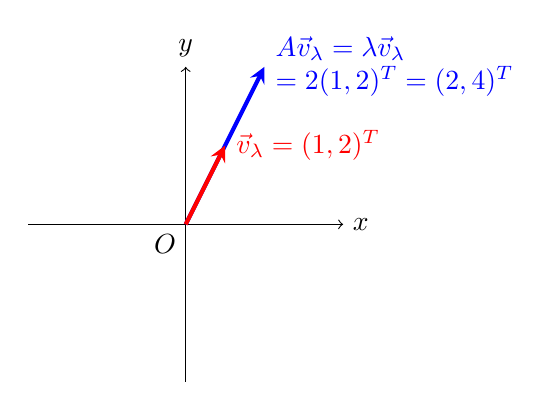
\begin{tikzpicture}
\draw[->] (-2,0)--(2,0) node[right]{$x$};
\draw[->] (0,-2)--(0,2) node[above]{$y$};
\draw[blue,-stealth,line width=1.5] (0,0)--(1,2) node[align=left, right]{$A\vec{v}_\lambda = \lambda\vec{v}_\lambda$\\ $= 2(1,2)^T = (2,4)^T$};
\draw[red,-stealth,line width=1.5] (0,0)--(1/2,1) node[anchor=west]{$\vec{v}_\lambda = (1,2)^T$};
\node[below left]{$O$}; 
\end{tikzpicture}
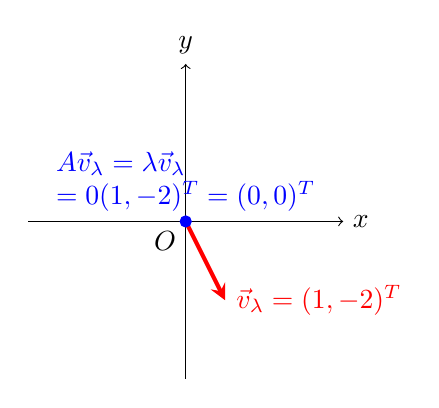
\begin{tikzpicture}
\draw[->] (-2,0)--(2,0) node[right]{$x$};
\draw[->] (0,-2)--(0,2) node[above]{$y$};
\draw[red,-stealth,line width=1.5] (0,0)--(1/2,-1) node[anchor=west]{$\vec{v}_\lambda = (1,-2)^T$};
\draw[blue, fill=blue] (0,0) circle[radius=2pt] node[align=left, above]{$A\vec{v}_\lambda = \lambda\vec{v}_\lambda$\\ $= 0(1,-2)^T = (0,0)^T$};
\node[below left]{$O$}; 
\end{tikzpicture}\\
Illustrations for the example above with $\lambda = 2 > 1$ (Extension), and $\lambda = 0$ (Vanished).
\end{center}
There are infinitely many eigenvectors which are oriented in the same direction for a single eigenvalue as seen in the remark of the last short exercise. Particularly, they are actually the span of any one of these eigenvectors that is non-zero. Thus, along a single direction, only one of them is needed for representation, and its span is at the same time a subspace by Properties \ref{proper:subspace_n_span}. This subspace is known as the \keywordhl{eigenspace} corresponding to that eigenvalue. Moreover, there may be more than one linearly independent eigenvectors for the same eigenvalue, and the dimension of eigenspace generated by them will be greater than one as well. In addition, the zero vector, technically, can be the eigenvectors of any matrix since $A\vec{0} = \vec{0} = \lambda\vec{0}$ for any matrix $A$ and scalar $\lambda$. However, it is a trivial solution, plus more importantly the zero vector is always linearly dependent by definition, and will not be taken into consideration (unlike the totally fine eigenvalue of zero).\\
\\
Below is the visualization of some other possibilities of eigenvector rescaling.
\begin{center}
\begin{tikzpicture}
\draw[->] (-1.5,0)--(1.5,0) node[right]{$x$};
\draw[->] (0,-1.5)--(0,1.5) node[above]{$y$};
\draw[red,-stealth] (0,0)--(0.75,1.5);
\draw[blue,-stealth] (0,0)--(0.25,0.5);
\node[below left]{$O$}; 
\end{tikzpicture}
\begin{tikzpicture}
\draw[->] (-1.5,0)--(1.5,0) node[right]{$x$};
\draw[->] (0,-1.5)--(0,1.5) node[above]{$y$};
\draw[red,-stealth] (0,0)--(1,-0.5);
\draw[blue,-stealth] (0,0)--(-0.8,0.4);
\node[below left]{$O$}; 
\end{tikzpicture}\\
Contraction ($0 < \lambda < 1$), Reversal ($\lambda < 0$). \\
\begin{tikzpicture}
\draw[->] (-1.5,0)--(1.5,0) node[right]{$x$};
\draw[->] (0,-1.5)--(0,1.5) node[above]{$y$};
\draw[Green,-stealth] (0,0)--(-1.25,1.25);
\node[below left]{$O$}; 
\end{tikzpicture}
\begin{tikzpicture}
\draw[->] (-1.5,0)--(1.5,0) node[right]{$x$};
\draw[->] (0,-1.5)--(0,1.5) node[above]{$y$};
\draw[red,-stealth] (0,0)--(1,1);
\draw[fill=blue] (0,0) circle[radius=2pt];
\node[below left]{$O$}; 
\end{tikzpicture}\\
Unchanged ($\lambda = 1$), Vanished ($\lambda = 0$). 
\end{center}

The eigenspace actually belongs to a broader class of subspaces known as the invariant subspaces.

\subsection{Finding Eigenvalues and Eigenvectors with Characteristic Polynomials}

To find eigenvalues, rearrange the equation in Definition \ref{eigen} relating eigenvalues and eigenvectors to obtain
\begin{align*}
A\vec{v}_\lambda &= \lambda\vec{v}_\lambda \\
A\vec{v}_\lambda &= \lambda I\vec{v}_\lambda  &\text{($I\vec{u} = \vec{u}$ for any $\vec{u}$)} \\
(A-\lambda I)\vec{v}_\lambda &= \vec{0}
\end{align*}
The last line constitutes a homogeneous linear system $B\vec{v}_\lambda = \vec{0}$ where $B = A - \lambda I$. For this system to have a non-trivial solution and hence an eigenvector, it is required that $\det(B) = \det(A - \lambda I) = 0$ from Theorem \ref{LinSysUnique}. The relationship $\det(A - \lambda I) = 0$ is called the characteristic equation. The roots for $\lambda$ of the characteristic polynomial are then the desired eigenvalues. \\
Short Exercise: By inspection, find all three eigenvalues of the matrix
\begin{align*}
\begin{bmatrix}
1 & 0 & 0 \\
0 & 2 & 0 \\
0 & 0 & 3
\end{bmatrix}
\end{align*}
For each eigenvalue there corresponds at least one eigenvectors. The number of eigenvectors for an eigenvalue depend on the number of the root appearing in the characteristic equation. The eigenvectors are then the general solution of the matrix equation $B\vec{v}_\lambda = (A - \lambda I)\vec{v}_\lambda = \vec{0}$, which exists because of the condition $\det(A - \lambda I) = 0$. The number of eigenvectors obeys the following theorem.
\begin{thm}
For each particular eigenvalue $\lambda_j$ for a matrix $A$ computed from its characteristic equation $\det(A - \lambda I) = 0$, the amount of $\lambda_j$ appearing as its root, or equivalently the power $n$ of the factor $(x-\lambda_j)^n$ in the characteristic polynomial, is called the algebraic multiplicity. \\
\\
Meanwhile, the amount of eigenvectors $\vec{v}_{\lambda_j}$ corresponding to $\lambda_j$ is called the geometric multiplicity. With these two quantities defined, we have
\begin{align*}
1 \leq \text{Geometric Multiplicity} \leq \text{Algebraic Multiplicity}
\end{align*}
for every eigenvalue $\lambda_j$.
\end{thm}

\begin{exmp}
Find all eigenvalues and eigenvectors for the matrix
\begin{align*}
A &=
\begin{bmatrix}
1 & -1 \\
0 & 1
\end{bmatrix}
\end{align*}
The characteristic equation is
\begin{align*}
\det(A - \lambda I) &= 
\begin{vmatrix}
1-\lambda & -1 \\
0 & 1-\lambda
\end{vmatrix} \\
&= (1-\lambda)^2 = 0
\end{align*}
Apparently, there is only one eigenvalue $\lambda = 1$, which has an algebraic multiplicity of $2$. Possible eigenvectors are then found by solving
\begin{align*}
\left[\begin{array}{@{}cc|c@{}}
1-1 & -1 & 0 \\
0 & 1-1 & 0
\end{array}\right] 
= 
\left[\begin{array}{@{}cc|c@{}}
0 & -1 & 0 \\
0 & 0 & 0
\end{array}\right]
\end{align*}
where the general solution is easily seen to be $t(1,0)^T$. So for the eigenvalue $\lambda = 1$, there is only one eigenvector $(1,0)^T$, which implies a geometric multiplicity of $1$.
\end{exmp}

\begin{exmp}
For the matrix
\begin{align*}
A &= 
\begin{bmatrix}
1 & 3 & 1 \\
0 & 1 & 0 \\
1 & 0 & 2
\end{bmatrix}
\end{align*}
the characteristic polynomial is
\begin{align*}
\begin{vmatrix}
1-\lambda & 3 & 1 \\
0 & 1-\lambda & 0 \\
1 & 0 & 2-\lambda 
\end{vmatrix} &=
(1-\lambda)(1-\lambda)(2-\lambda) - (1)(1-\lambda)(1) \\
&= (1-\lambda)((2-3\lambda+\lambda^2) - 1) \\
&= (1-\lambda)(1-3\lambda+\lambda^2)
\end{align*}
The roots and thus eigenvalues are $\lambda = 1$, as well as
\begin{align*}
\lambda &= \frac{-(-3) \pm \sqrt{(-3)^2 - 4(1)(1)}}{2} \\
&= \frac{3}{2} \pm \frac{\sqrt{5}}{2}
\end{align*}
Particularly, for the eigenvalue $\lambda = \frac{3}{2} + \frac{\sqrt{5}}{2}$, the eigenvector is inferred from the homogeneous system
\begin{align*}
\left[\begin{array}{@{}ccc|c@{}}
-\frac{1}{2}-\frac{\sqrt{5}}{2} & 3 & 1 & 0 \\
0 & -\frac{1}{2}-\frac{\sqrt{5}}{2} & 0 & 0 \\
1 & 0 & \frac{1}{2}-\frac{\sqrt{5}}{2} & 0
\end{array}\right] &\to
\left[\begin{array}{@{}ccc|c@{}}
1 & 0 & \frac{1}{2}-\frac{\sqrt{5}}{2} & 0 \\
0 & 1 & 0 & 0 \\
-\frac{1}{2}-\frac{\sqrt{5}}{2} & 3 & 1 & 0
\end{array}\right]  \\
&\to
\left[\begin{array}{@{}ccc|c@{}}
1 & 0 & \frac{1}{2}-\frac{\sqrt{5}}{2} & 0 \\
0 & 1 & 0 & 0 \\
0 & 0 & 0 & 0
\end{array}\right]
\end{align*}
whose general solution and hence the eigenvector is $(-\frac{1}{2}+\frac{\sqrt{5}}{2},0,1)^T$ for $\lambda = \frac{3}{2} + \frac{\sqrt{5}}{2}$.\\
Short Exercise: Find the eigenvectors for other remaining eigenvalues.
\end{exmp}

This section is ended with some notable properties of eigenvalue and eigenvector.
\begin{proper}
For a square matrix $A$,
\begin{enumerate}
\item $A^T$ shares the same eigenvalues, but for each eigenvalue the eigenvector is not guaranteed to be the same,
\item The eigenvalues for the inverse $A^{-1}$, provided that it exists, are the reciprocals of the eigenvalues of $A$, but the eigenvectors are the same. This can be proved by starting with $A\vec{v}_\lambda = \lambda\vec{v}_\lambda$, and multiplying to the left on both sides by $A^{-1}$.
\end{enumerate}
\end{proper}

\subsection*{Cayley-Hamilton Theorem}
Here we introduce an important theorem, Cayley-Hamilton Theorem, stating that, for every square matrix, it satisfies its own characteristic equation, which means that substituting the matrix into the characteristic polynomial as the variable results in a zero matrix.
\begin{thm}
By Cayley-Hamilton Theorem, for any $n \times n$ square matrix $A$, if the characteristic polynomial is
\begin{align*}
p(\lambda) = \det(A-\lambda I) = \sum_{k=0}^{n} c_k \lambda^k
\end{align*}
then we have
\begin{align*}
p(A) = \sum_{k=0}^{n} c_k A^k = [\textbf{0}]
\end{align*}
which is a $n \times n$ zero matrix.
\end{thm}
One may be tempted to substitute $\lambda = A$ into $\det(A-\lambda I)$ to prove the Cayley-Hamilton Theorem. However, since $\lambda$ is a scalar but $A$ is a matrix, it is not a rigorous proof. Correct proofs require advanced knowledge, which will not be presented here.

\begin{exmp}
With the matrix
\begin{align*}
A = 
\begin{bmatrix}
1 & -1 \\
3 & 5
\end{bmatrix}
\end{align*}
verify the Cayley-Hamilton Theorem, and use the Cayley-Hamilton Theorem to evaluate $A^2 - 7A + 6I$.\\
\\
The characteristic polynomial is
\begin{align*}
\begin{vmatrix}
1-\lambda & -1 \\
3 & 5-\lambda
\end{vmatrix}  
&= (1-\lambda)(5-\lambda) - (3)(-1) \\
&= 5 - 6 \lambda + \lambda^2 + 3 \\
&= \lambda^2 - 6\lambda + 8
\end{align*}
Replacing all $\lambda^k$ terms in the characteristic polynomial with $A^k$ (Notice that the constant term $c_0$ becomes $c_0 I$), we have
\begin{align*}
A^2 - 6A + 8I &= 
\begin{bmatrix}
1 & -1 \\
3 & 5
\end{bmatrix}^2
- 6
\begin{bmatrix}
1 & -1 \\
3 & 5
\end{bmatrix} 
+ 8
\begin{bmatrix}
1 & 0 \\
0 & 1
\end{bmatrix} \\
&=
\begin{bmatrix}
-2 & -6 \\
18 & 22
\end{bmatrix}
+
\begin{bmatrix}
-6 & 6 \\
-18 & -30
\end{bmatrix} 
+
\begin{bmatrix}
8 & 0 \\
0 & 8
\end{bmatrix} \\
&=
\begin{bmatrix}
0 & 0\\
0 & 0
\end{bmatrix}
\end{align*}
So Cayley-Hamilton Theorem holds in this case. We can quickly compute $A^2 - 7A + 6I$ by
\begin{align*}
A^2 - 7A + 6I &= (A^2 - 7A + 6I) - (A^2 - 6A + 8I) \\
&= -A-2I \\
&= -\begin{bmatrix}
1 & -1 \\
3 & 5
\end{bmatrix} 
-2
\begin{bmatrix}
1 & 0 \\
0 & 1
\end{bmatrix} \\
&=
\begin{bmatrix}
-3 & 1 \\
-3 & -7
\end{bmatrix}
\end{align*}
since $A^2 - 6A + 8I$ is a zero matrix.
\end{exmp}

\section{Diagonalization}

\subsection{Ideas and Properties of Diagonalization}
The properties of eigenvectors allow us to carry out diagonalization which helps us to solve linear algebra related problem. A matrix $P$ is said to diagonalize another matrix $A$ if the product $P^{-1}AP$ results in a diagonal matrix $D$, where non-zero entries are only found along the main diagonal.
\begin{defn}
A square matrix $A$ is diagonalizable, if there exists some invertible square matrix $P$, such that
\begin{align*}
P^{-1}AP = D
\end{align*}
where $D$ is a diagonal matrix.
\end{defn}
Particularly, the matrix $P$ required for diagonalizing matrix $A$ is formed by combining all the eigenvectors of $A$ column by column. This is only possible if the amount of distinct eigenvectors is equal to the size of A.
\begin{proper}
\label{diagonalize}
A $n \times n$ square matrix $A$ can be diagonalized by another matrix $P$, if $A$ has $n$ linearly independent eigenvectors, and the column vectors of $P$ are those eigenvectors. A equivalent condition is that for every eigenvalue, its geometric multiplicity is equal to the algebraic multiplicity. The diagonal entries of $P^{-1}AP = D$, are the eigenvalues $\lambda_j$ corresponding to the eigenvectors $\vec{v}_{\lambda_j}$ in the same column of $P$. 
\paragraph{Proof}
Consider two matrix dot products $AP$ and $PD$, where $P = [\vec{v}_{\lambda_1}|\cdots|\vec{v}_{\lambda_n}]$
\begin{align*}
AP &= A[\vec{v}_{\lambda_1}|\cdots|\vec{v}_{\lambda_n}] \\
&= [A\vec{v}_{\lambda_1}|\cdots|A\vec{v}_{\lambda_n}] \\
&= [\lambda_1\vec{v}_{\lambda_1}|\cdots|\lambda_n \vec{v}_{\lambda_n}]
\end{align*}
where we have used the Definition \ref{eigen} and the second step can be compared to the last paragraph in Section \ref{6.1.1}. Also
\begin{align*}
PD &= [\vec{v}_{\lambda_1}|\cdots|\vec{v}_{\lambda_n}]
\begin{bmatrix}
\lambda_1 & \cdots & 0 \\
\vdots & \ddots & \vdots \\
0 & \cdots & \lambda_n
\end{bmatrix} \\
&= [\lambda_1\vec{v}_{\lambda_1}|\cdots|\lambda_n \vec{v}_{\lambda_n}]
\end{align*}
So $AP = PD$. Notice that $P$ is invertible by Theorem \ref{equiv3}, since $P$ is made up of linearly independent eigenvectors, and thus $P^{-1}AP = D$.
\end{proper}

The original matrix $A$ and its diagonalization form $P^{-1}AP$ share some similarities sometimes called invariants. 
\begin{proper}
If there are a diagonalizable matrix $A$, and its diagonalization form $D = P^{-1}AP$, then $A$ and $D$ have the
\begin{enumerate}
\item Same determinant, 
\item Same trace, 
\item Same eigenvalues, 
\item Same characteristic equation.
\end{enumerate}
\end{proper}
Short Exercise: Prove the invariant property for determinant.

\subsection{Diagonalization for Real Eigenvalues}

For a diagonalizable matrix with real eigenvalues, diagonalization is straight forward by the use of Properties \ref{diagonalize}. Below shows a simple example.
\begin{exmp}
For the matrix 
\begin{align*}
A &= 
\begin{bmatrix}
3 & -1 & 1 \\
-2 & 4 & 2 \\
-1 & 1 & 5
\end{bmatrix}
\end{align*}
It is given that its eigenvectors are $(1,1,0)^T, (1,0,1)^T, (0,1,1)^T$ for $\lambda = 2,4,6$ respectively. Concatenating them column by column yields
\begin{align*}
P &=
\begin{bmatrix}
1 & 1 & 0 \\
1 & 0 & 1 \\
0 & 1 & 1
\end{bmatrix}
\end{align*}
The matrix product
\begin{align*}
D &= P^{-1}AP \\
&=
\begin{bmatrix}
1 & 1 & 0 \\
1 & 0 & 1 \\
0 & 1 & 1
\end{bmatrix}^{-1}
\begin{bmatrix}
3 & -1 & 1 \\
-2 & 4 & 2 \\
-1 & 1 & 5
\end{bmatrix}
\begin{bmatrix}
1 & 1 & 0 \\
1 & 0 & 1 \\
0 & 1 & 1
\end{bmatrix} \\
&=
\begin{bmatrix}
\frac{1}{2} & \frac{1}{2} & -\frac{1}{2} \\
\frac{1}{2} & -\frac{1}{2} & \frac{1}{2} \\
-\frac{1}{2} & \frac{1}{2} & \frac{1}{2}
\end{bmatrix}
\begin{bmatrix}
2 & 4 & 0 \\
2 & 0 & 6 \\
0 & 4 & 6
\end{bmatrix} \\
&=
\begin{bmatrix}
2 & 0 & 0 \\
0 & 4 & 0 \\
0 & 0 & 6
\end{bmatrix}
\end{align*}
This is expected from Properties \ref{diagonalize}.\\
Short Exercise: Confirm the provided eigenvalues and eigenvectors. Also, reverse the diagonalization to recover the original matrix.\\
Short Exercise: Verify the invariant properties for this example.
\end{exmp}

\subsection{Diagonalization for Complex Eigenvalues}
It is not uncommon for a real square matrix $A$ to have complex eigenvalues. In such cases, to perform diagonalization, one possible approach is following what we have done in the last section to generate $D = P^{-1}AP$, which can be useful sometimes, but the downsides are that $P$ and $D$ are comprised of complex numbers, despite $A$ being a real matrix. There is, indeed, another method uses the property of complex numbers introduced in the last chapter, that avoids the appearance of complex numbers. But first of all, we need to introduce a basic theorem about complex roots of an equation.
\begin{thm}
For a real polynomial equation with order $n$
\begin{align*}
p(x) = \sum_{k=0}^{n} c_k x^k
\end{align*}
If $x_0 = a+b\imath$ is a complex root so that $p(x_0) = \sum_{k=0}^{n} c_k x_0^k = 0$, where $a$ and $b$ are real constants, then
$\overline{x_0} = a-b\imath$ is also a root for the equation.
\paragraph{Proof}
By Properties \ref{complexnum}, if we take the complex conjugate on both sides of the polynomial equation with $x = x_0$, then
\begin{align*}
\overline{p(x_0)} &= \overline{\sum_{k=0}^{n} c_k x_0^k} = \overline{0} \\
{p(\overline{x_0})} &= \sum_{k=0}^{n} c_k \overline{x_0}^k = 0
\end{align*}
\end{thm}
Since the characteristic equation is a real polynomial equation for the real matrix $A$, by the theorem we have just proved, we know that complex roots for the characteristic equation and hence complex eigenvalues always come in a conjugate pair. For a pair of complex eigenvalues, their eigenvectors are also the conjugate of each other.
\begin{proper}
If $\lambda_0$ is an eigenvalue for a real matrix $A$ with an eigenvector of $\vec{v}_{\lambda_0}$, then $A$ also has $\overline{\lambda_0}$ and $\overline{\vec{v}_{\lambda_0}}$ as another eigenvalue and eigenvector.
\paragraph{Proof}
By definition,
\begin{align*}
A\vec{v}_{\lambda_0} &= \lambda_0\vec{v}_{\lambda_0}    
\end{align*}
Taking complex conjugate on both sides, we have
\begin{align*}
\overline{A\vec{v}_{\lambda_0}} &= \overline{\lambda_0\vec{v}_{\lambda_0}} \\
A \overline{\vec{v}_{\lambda_0}} &= \overline{\lambda_0}\; \overline{\vec{v}_{\lambda_0}}
\end{align*}
with the use of Properties \ref{complexnum}, and noting that $\overline{A} = A$ as $A$ is a real matrix.
\end{proper}
Now as we know that complex eigenvalues and eigenvectors always appear as a pair of complex conjugates, and conjugates share the same real and imaginary part except a sign difference, we are encouraged to use their real and imaginary part like two eigenvalues and eigenvectors for making up. The following theorem shows that it is possible to do so with some tweaks.

\begin{thm}
\label{diagonalize2}
The procedure in Properties \ref{diagonalize} can be extended for complex eigenvalue $\lambda_0 = \Re{\lambda_0} + \imath \Im{\lambda_0}$, the corresponding eigenvector $\vec{v}_{\lambda_0} = \Re{\vec{v}_{\lambda_0}} + \imath \Im{\vec{v}_{\lambda_0}}$, as well as their complex conjugates, by replacing the corresponding columns in
\begin{align*}
&P = [\cdots|\vec{v_{\lambda_0}}|\overline{\vec{v_{\lambda_0}}}|\cdots]
&D =
\begin{bmatrix}
\ddots & 0 & 0 & \\
& \lambda_0 & 0 & \\
& 0 & \overline{\lambda_0} & \\
& 0 & 0 & \ddots
\end{bmatrix}
\end{align*}
by
\begin{align*}
&P = [\cdots|\Re{\vec{v}_{\lambda_0}}|\Im{\vec{v}_{\lambda_0}}|\cdots]
&D =
\begin{bmatrix}
\ddots & 0 & 0 & \\
& \Re{\lambda_0} & -\Im{\lambda_0} & \\
& \Im{\lambda_0} & \Re{\lambda_0} & \\
& 0 & 0 & \ddots
\end{bmatrix}
\end{align*}
\paragraph{Proof}
As in the proof for Properties \ref{diagonalize}, we set to prove that $AP = PD$ for the columns concerned. To make it easier to read, denote $\Re{\lambda_0} = a$ and $\Im{\lambda_0} = b$. It is easy to see that
\begin{align*}
PD &=
[\cdots|\Re{\vec{v}_{\lambda_0}}|\Im{\vec{v}_{\lambda_0}}|\cdots]
\begin{bmatrix}
\ddots & 0 & 0 & \\
& a & b & \\
& -b & a & \\
& 0 & 0 & \ddots
\end{bmatrix} \\
&= [\cdots|a\Re{\vec{v}_{\lambda_0}} - b\Im{\vec{v}_{\lambda_0}} | b\Re{\lambda_0} + a\Im{\vec{v}_{\lambda_0}}|\cdots]
\end{align*}
Notice that the relation between eigenvalue and eigenvector can be expanded as
\begin{align*}
A\vec{v}_{\lambda_0} &= \lambda_0\vec{v}_{\lambda_0} \\
A(\Re{\vec{v}_{\lambda_0}} + \imath \Im{\vec{v}_{\lambda_0}}) &= (a+b\imath)(\Re{\vec{v}_{\lambda_0}} + \imath \Im{\vec{v}_{\lambda_0}}) \\
A\Re{\vec{v}_{\lambda_0}} + \imath A\Im{\vec{v}_{\lambda_0}} &= (a\Re{\vec{v}_{\lambda_0}} - b\Im{\vec{v}_{\lambda_0}}) + \imath(b\Re{\vec{v}_{\lambda_0}} + a\Im{\vec{v}_{\lambda_0}})
\end{align*}
By equating real and imaginary parts, we have
\begin{align*}
A\Re{\vec{v}_{\lambda_0}} &= a\Re{\vec{v}_{\lambda_0}} - b\Im{\vec{v}_{\lambda_0}} \\
A\Im{\vec{v}_{\lambda_0}} &= b\Re{\vec{v}_{\lambda_0}} + a\Im{\vec{v}_{\lambda_0}}
\end{align*}
Hence
\begin{align*}
AP &= A[\cdots|\Re{\vec{v}_{\lambda_0}}|\Im{\vec{v}_{\lambda_0}}|\cdots] \\
&= [\cdots|A\Re{\vec{v}_{\lambda_0}}|A\Im{\vec{v}_{\lambda_0}}|\cdots] \\
&= [\cdots|a\Re{\vec{v}_{\lambda_0}} - b\Im{\vec{v}_{\lambda_0}} | b\Re{\lambda_0} + a\Im{\vec{v}_{\lambda_0}}|\cdots] \\
&= PD
\end{align*}
The only caveat is to prove that $P$ is invertible, or equivalently $\Re{\vec{v}_{\lambda_0}}$ and $\Im{\vec{v}_{\lambda_0}}$ are linearly independent. We can prove that by assuming they are linearly dependent, so $\Re{\vec{v}_{\lambda_0}} = k\Im{\vec{v}_{\lambda_0}}$ for some $k$, and plugging this into the expressions of $A\Re{\vec{v}_{\lambda_0}}$ and $A\Im{\vec{v}_{\lambda_0}}$ to derive a contradiction.
\end{thm}

The block in the form
\begin{align*}
\begin{bmatrix}
\ddots & 0 & 0 & \\
& a & b & \\
& -b & a & \\
& 0 & 0 & \ddots
\end{bmatrix}    
\end{align*}
generally represents a rotation by a degree of $\theta = \arctan(b/a)$. It means that a complex eigenvalue entails a rotation. This will be discussed more thoroughly in the next chapter.

\begin{exmp}
\label{ex8.2.2}
Using Theorem \ref{diagonalize2} to convert
\begin{align*}
A &= 
\begin{bmatrix}
1 & 1 \\
-2 & 1
\end{bmatrix}
\end{align*}
into the form $D = P^{-1}AP$.\\
The characteristic equation is
\begin{align*}
\begin{bmatrix}
1-\lambda & 1 \\
-2 & 1-\lambda
\end{bmatrix} 
&=
(1-\lambda)^2 + 2 \\
&= \lambda^2 - 2\lambda + 3 = 0
\end{align*}
The roots are
\begin{align*}
\lambda &= \frac{-(-2) \pm \sqrt{(-2)^2 - 4(1)(3)}}{2} \\
&= 1 \pm \sqrt{2}\imath
\end{align*}
Since the eigenvectors occur in a conjugate pair, we only need to find one of them. We can find the eigenvector for $\lambda = 1 - \sqrt{2}\imath$, by solving the system
\begin{align*}
\left[\begin{array}{@{}cc|c@{}}
\sqrt{2}\imath & 1 & 0 \\
-2 & \sqrt{2}\imath & 0
\end{array}\right] &\to  
\left[\begin{array}{@{}cc|c@{}}
\sqrt{2}\imath & 1 & 0 \\
0 & 0 & 0
\end{array}\right]
\end{align*}
So the eigenvector for $\lambda = 1 - \sqrt{2}\imath$ is $(\imath, \sqrt{2})^T$, and the eigenvector for $\lambda = 1 + \sqrt{2}\imath$ is $(-\imath, \sqrt{2})^T$.
Applying Theorem \ref{diagonalize2}, with $a = 1$, $b = \sqrt{2}$, $\Re{\vec{v}_{\lambda_0}} = (0,\sqrt{2})^T$, $\Im{\vec{v}_{\lambda_0}} = (-1,0)^T$, we have
\begin{align*}
\begin{bmatrix}
1 & \sqrt{2} \\
-\sqrt{2} & 1
\end{bmatrix}
&= 
\begin{bmatrix}
0 & -1 \\
\sqrt{2} & 0
\end{bmatrix}^{-1}
\begin{bmatrix}
1 & 1 \\
-2 & 1
\end{bmatrix}
\begin{bmatrix}
0 & -1 \\
\sqrt{2} & 0
\end{bmatrix}
\end{align*}
\end{exmp}

\section{System of Ordinary Differential Equations}
Ordinary Differential Equations appear frequently in the area of Physics and Earth Science. The easiest class of Ordinary Differential Equations is the first-order, linear, homogeneous Ordinary Differential Equations.
\begin{defn}
A first-order linear ordinary differential equation is a differential equation in the form of
\begin{align*}
\frac{dy}{dx} + P(x)y = Q(x)
\end{align*}
where $x$ is the indepedent variable, $y(x)$ is the dependent variable, $P(x)$ and $Q(x)$ is some function of $x$. 
\end{defn}
First-order means that the highest order derivative involved is the first derivative. Linearity means that there are no cross product terms between the dependent variable and its derivatives, e.g. $y\frac{dy}{dx}, y^2$. Finally, if it is of constant coefficients, and homogeneous, then it implies that $P(x)$ is a constant and $Q(x) = 0$ respectively.
\begin{thm}
\label{ODEsol}
For a first-order, linear, constant coefficients, homogenenous ordinary differential equation in the form of
\begin{align*}
\frac{dy}{dx} = \beta y
\end{align*}
where $\beta$ is a constant, the general solution is
\begin{align*}
y(x) = ce^{\beta x}
\end{align*}
with $c$ as the integration constant. A direct substitution can verify the solution.
\end{thm}
However, for some real-life problems, there are multiple ordinary differential equations that are related to each other to be solved. This especially happens in the area of Earth System Science where we have to consider the interactions, such as mass flow, between different units. This gives rise to a system of ordinary differential equations.
\begin{defn}
A system of ordinary differential equations that are first-order, linear, constant coefficients, and homogeneous has the form of
\begin{align*}
\begin{cases}
dy_1/dx &= \alpha_1 y_1 + \beta_1 y_2 + \gamma_1 y_3 + \cdots \\
dy_2/dx &= \alpha_2 y_1 + \beta_2 y_2 + \gamma_2 y_3 + \cdots \\
dy_3/dx &= \alpha_3 y_1 + \beta_3 y_2 + \gamma_3 y_3 + \cdots \\
\cdots &= \cdots
\end{cases}
\end{align*}
and so on, up to $dy_n/dx$, or more compactly
\begin{align*}
\frac{dy_i}{dx} &= \alpha_i y_1 + \beta_i y_2 + \gamma_i y_3 + \cdots
\end{align*}
or in matrix notation
\begin{align*}
\textbf{y}' &= A\textbf{y}
\end{align*}
where $\alpha_i, \beta_i, \gamma_i, \cdots$ are constants, $A$ is a square $n \times n$ matrix, and
\begin{align*}
&\textbf{y} =
\begin{bmatrix}
y_1 \\
y_2 \\
y_3
\end{bmatrix}
&\textbf{y}' =
\begin{bmatrix}
dy_1/dx \\
dy_2/dx \\
dy_3/dx
\end{bmatrix} \\
&A=
\begin{bmatrix}
\alpha_1 & \beta_1 & \gamma_1 & \cdots \\
\alpha_2 & \beta_2 & \gamma_2 & \\
\alpha_3 & \beta_3 & \gamma_3 &  \\
\vdots & & & \ddots
\end{bmatrix}
\end{align*}
\end{defn}
An example is the system
\begin{align*}
\begin{cases}
dy_1/dx &= 3y_1 - y_2 \\
dy_2/dx &= 2y_1
\end{cases} 
\end{align*}
which can be rewritten into
\begin{align*}
\textbf{y}' =
\begin{bmatrix}
3 & -1 \\
2 & 0
\end{bmatrix}
\textbf{y}
\end{align*}
Since each ordinary differential equations for $dy_i/dx$ now involves multiple dependent variables $y_j$, where $j = 1,2,3,\cdots$, at the right hand side, we cannot directly use the result from Theorem \ref{ODEsol} to solve the system, unless we can find a way to transform the system so that each equation is in terms of a single dependent variable only. Notice that if we make a change of variables such that $\textbf{y} = P\textbf{z}$ and hence $\textbf{y}' = P\textbf{z}'$, then the system $\textbf{y}' = A\textbf{y}$ becomes
\begin{align*}
P\textbf{z}' &= AP\textbf{z} \\
\textbf{z}' &= (P^{-1}AP)\textbf{z}
\end{align*}
if we assume $P$ is invertible. The term $P^{-1}AP$ immediately tells us a hint in the sense that it resembles a diagonalization described in \ref{diagonalize}. If $P^{-1}AP = D$, which is a diagonal matrix, then the system becomes $\textbf{z}' = D\text{z}$, written more explicitly, is
\begin{align*}
\begin{cases}
dz_1/dx &= D_{11}z_1 \\
dz_2/dx &= D_{22}z_2 \\
dz_3/dx &= D_{33}z_3 \\
\cdots &= \cdots
\end{cases}     
\end{align*}
which are all solvable in their own. Subsequently, we have the following conclusion.
\begin{thm}
For a system of ordinary differential equations in the form of 
\begin{align*}
\textbf{y}' &= A\textbf{y}
\end{align*}
where $A$ is a square $n \times n$ matrix with constant entries, it is solvable if $A$ is diagonalizable, and we make the change of variables
\begin{align*}
\textbf{y} = P\textbf{z}
\end{align*}
where $P$ is the eigenvector matrix outlined in Properties \ref{diagonalize}. So that the system becomes
\begin{align*}
\textbf{z}' &= (P^{-1}AP)\textbf{z} = D\textbf{z}
\end{align*}
After solving for $\textbf{z}$, we can recover the required solution by computing $\textbf{y} = P\textbf{z}$.
\end{thm}

\begin{exmp}
Solve the following system of differential equations.
\begin{align*}
\begin{cases}
dy_1/dx &= \frac{5}{2} y_1 + y_2 + \frac{1}{2} y_3 \\
dy_2/dx &= \frac{3}{2} y_1 + 3 y_2 - \frac{1}{2} y_3 \\
dy_3/dx &= \frac{3}{2} y_1 + y_2 + \frac{3}{2} y_3 
\end{cases}    
\end{align*}
The system written in matrix notation is
\begin{align*}
\begin{bmatrix}
dy_1/dx \\
dy_2/dx \\
dy_3/dx
\end{bmatrix}
=
\begin{bmatrix}
\frac{5}{2} & 1 & \frac{1}{2} \\
\frac{3}{2} & 3 & -\frac{1}{2} \\
\frac{3}{2} & 1 & \frac{3}{2}
\end{bmatrix}
\begin{bmatrix}
y_1 \\
y_2 \\
y_3
\end{bmatrix}
\end{align*}
We leave to the readers to check that the eigenvectors for the coefficient matrix are $(-1,1,1)^T$, $(1,-1,1)^T$, $(1,1,1)^T$ for $\lambda = 1, 2, 4$. Hence by the theorem we have just derived, we can make the change of variables
\begin{align*}
\begin{bmatrix}
y_1 \\
y_2 \\
y_3
\end{bmatrix}
=
\begin{bmatrix}
-1 & 1 & 1 \\
1 & -1 & 1 \\
1 & 1 & 1
\end{bmatrix}
\begin{bmatrix}
z_1 \\
z_2 \\
z_3
\end{bmatrix}
\end{align*}
so that the system becomes
\begin{align*}
\begin{bmatrix}
dz_1/dx \\
dz_2/dx \\
dz_3/dx
\end{bmatrix}
&=
\begin{bmatrix}
-1 & 1 & 1 \\
1 & -1 & 1 \\
1 & 1 & 1
\end{bmatrix}^{-1}
\begin{bmatrix}
\frac{5}{2} & 1 & \frac{1}{2} \\
\frac{3}{2} & 3 & -\frac{1}{2} \\
\frac{3}{2} & 1 & \frac{3}{2}
\end{bmatrix}
\begin{bmatrix}
-1 & 1 & 1 \\
1 & -1 & 1 \\
1 & 1 & 1
\end{bmatrix}
\begin{bmatrix}
z_1 \\
z_2 \\
z_3
\end{bmatrix} \\
&=
\begin{bmatrix}
1 & 0 & 0\\
0 & 2 & 0\\
0 & 0 & 4
\end{bmatrix}
\begin{bmatrix}
z_1 \\
z_2 \\
z_3
\end{bmatrix}
\end{align*}
The solution in terms of $z_i$ is $z_1 = c_1e^x$, $z_2 = c_2e^{2x}$, $z_3 = c_3e^{4x}$. The integration constants $c_i$ can be determined by the so-called initial condition. Assume that the initial condition reads $y_1 = 3$, $y_2 = 1$, $y_3 = 5$, for $x = 0$, then substitution into the change of variables gives
\begin{align*}
\begin{bmatrix}
y_1(0) \\
y_2(0) \\
y_3(0)
\end{bmatrix}
&=
\begin{bmatrix}
-1 & 1 & 1 \\
1 & -1 & 1 \\
1 & 1 & 1
\end{bmatrix}
\begin{bmatrix}
z_1(0) \\
z_2(0) \\
z_3(0)
\end{bmatrix} \\
\begin{bmatrix}
3 \\
1 \\
5
\end{bmatrix}
&=
\begin{bmatrix}
-1 & 1 & 1 \\
1 & -1 & 1 \\
1 & 1 & 1
\end{bmatrix}
\begin{bmatrix}
c_1 \\
c_2 \\
c_3
\end{bmatrix}
\end{align*}
It is not hard to see that $c_1 = 1$, $c_2 = 2$, $c_3 = 2$, $z_1 = e^x$, $z_2 = 2e^{2x}$, $z_3 = 2e^{4x}$. So the full solution for $y_i$ is
\begin{align*}
\begin{cases}
y_1 &= -e^{x} + 2e^{2x} + 2e^{4x} \\
y_2 &= e^{x} - 2e^{2x} + 2e^{4x} \\
y_3 &= e^{x} + 2e^{2x} + 2e^{4x}
\end{cases}
\end{align*}
or in vector notation
\begin{align*}
\begin{bmatrix}
y_1 \\
y_2 \\
y_3
\end{bmatrix}
=
e^{x}
\begin{bmatrix}
-1 \\
1 \\
1
\end{bmatrix}
+
e^{2x}
\begin{bmatrix}
2 \\
-2 \\
2
\end{bmatrix}
+
e^{4x}
\begin{bmatrix}
2 \\
2 \\
2
\end{bmatrix}
\end{align*}
Short Exercise: Derive another solution if the initial condition is $y_1(x=0) = 0$, $y_2(x=0) = 4$, $y_3(x=0) = 6$ instead.
\end{exmp}

\begin{exmp}
Solve the system $\textbf{y}' = A\textbf{y}$, where
\begin{align*}
A = 
\begin{bmatrix}
1 & 1 \\
-2 & 1
\end{bmatrix}    
\end{align*}
is given in Example \ref{ex8.2.2}.\\
\\
From the previous work we know that the eigenvectors are $(\imath,\sqrt{2})^T$ and $(-\imath,\sqrt{2})^T$ for $\lambda = 1-\sqrt{2}\imath, 1+\sqrt{2}\imath$ respectively. In this situation it is advantageous to work with complex numbers as we will see soon. Similar to the example above, letting $\textbf{y} = P\textbf{z}$, where
\begin{align*}
P &=
\begin{bmatrix}
\imath & -\imath \\
\sqrt{2} & \sqrt{2} 
\end{bmatrix}
\end{align*}
then we have
\begin{align*}
\textbf{z}' &= (P^{-1}AP)\textbf{z} = D\textbf{z}
\end{align*}
with 
\begin{align*}
D &=
\begin{bmatrix}
1 - \sqrt{2}\imath & 0 \\
0 & 1 + \sqrt{2}\imath
\end{bmatrix}
\end{align*}
The solution in Theorem \ref{ODEsol} is valid even when $\beta$ is complex. Hence the solution for $z$ will be
\begin{align*}
\begin{cases}
z_1 &= c_1e^{(1-\sqrt{2}\imath)x} = c_1e^{x}(\cos(\sqrt{2}x) - \imath\sin\sqrt{2}x)\\
z_2 &= c_2e^{(1+\sqrt{2}\imath)x} = c_2e^{x}(\cos(\sqrt{2}x) + \imath\sin\sqrt{2}x)
\end{cases}
\end{align*}
where Euler's formula from Definition \ref{Euler} is applied. Hence 
\begin{align*}
\begin{bmatrix}
y_1 \\
y_2
\end{bmatrix}
&=
\begin{bmatrix}
\imath & -\imath \\
\sqrt{2} & \sqrt{2} 
\end{bmatrix}
\begin{bmatrix}
c_1e^{x}(\cos(\sqrt{2}x) - \imath\sin(\sqrt{2}x)) \\
c_2e^{x}(\cos(\sqrt{2}x) + \imath\sin(\sqrt{2}x))
\end{bmatrix} \\
&= 
\begin{bmatrix}
(c_1 + c_2)e^{x}\sin(\sqrt{2}x) + \imath(c_1-c_2)e^{x}\cos(\sqrt{2}x) \\
\sqrt{2}(c_1+c_2)e^{x}\cos(\sqrt{2}x) - \imath\sqrt{2}(c_1-c_2)e^{x}\sin(\sqrt{2}x)
\end{bmatrix} \\
&= 
\begin{bmatrix}
C_1e^{x}\sin(\sqrt{2}x) + \imath C_2e^{x}\cos(\sqrt{2}x) \\
\sqrt{2}C_1e^{x}\cos(\sqrt{2}x) - \imath \sqrt{2}C_2e^{x}\sin(\sqrt{2}x)
\end{bmatrix}
\end{align*}
if we write $C_1 = c_1 + c_2$, $C_2 = c_1 - c_2$. Both the real and imaginary parts of $\textbf{y}$ will satisfy the system, and they form the general solution. It is because $A$ is a real matrix, hence we can rewrite
\begin{align*}
\vec{y'} &= A\vec{y} \\
\Re{\vec{y'}} + \imath\Im{\vec{y'}} &= A(\Re{\vec{y}} + \imath\Im{\vec{y}}) \\
\Re{\vec{y'}} + \imath\Im{\vec{y'}} &= A\Re{\vec{y}} + \imath A\Im{\vec{y}}
\end{align*}
Equating the real and imaginary parts gives
\begin{align*}
\vec{y'}_{Re} &= A\vec{y}_{Re} \\
\vec{y'}_{Im} &= A\vec{y}_{Im}
\end{align*}
So the final answer, expressed in real values, is
\begin{align*}
\begin{cases}
y_1 &= C_1e^{x}\sin(\sqrt{2}x) + C_2e^{x}\cos(\sqrt{2}x) \\
y_2 &= \sqrt{2}C_1e^{x}\cos(\sqrt{2}x) - \sqrt{2}C_2e^{x}\sin(\sqrt{2}x)
\end{cases}
\end{align*}
where $C_1, C_2$ are to be decided by initial condition.
\end{exmp}
This will be the same solution basis we will obtain if we consider only one eigenvalue $\lambda_0$ out of the conjugate pair and compute $\vec{y} = \vec{v}_{\lambda_0}e^{\lambda_0 x}$. 

\section{Invariant Subspaces, Cayley-Hamilton Theorem}

\paragraph{Remark} If the coefficient matrix for a system of ordinary differential equation is not diagonalizable, then we need to employ other methods to solve the system. The most common method, generalized from diagonalization, is the Jordan Normal Form. Interested readers are invited to search about it.

\section{Earth Science Applications}

\section{Python Programming}

\section{Exercises}

\begin{Exercise}
If a matrix $A$ has a determinant of zero, show that it must have $\lambda = 0$ as an eigenvalue.
\end{Exercise}

\begin{Exercise}
Show that if the eigenvalues of a matrix $A$ all have an algebraic multiplicity of $1$, or in other words, no repeated root for the characteristic equation, then $A$ is diagonalizable. 
\end{Exercise}

\begin{Exercise}
Find the eigenvalues of the following matrices.
\begin{align*}
&A =
\begin{bmatrix}
1 & 3 & 3\\
4 & 0 & 4\\
0 & 1 & 2
\end{bmatrix}
&B =
\begin{bmatrix}
1 & 2 & 3 & 4\\
0 & 5 & 6 & 7\\
0 & 0 & 8 & 9\\
0 & 0 & 0 & 10
\end{bmatrix}
\end{align*}
as well as their transpose.
\end{Exercise}

\begin{Exercise}
Find the eigenvalues and corresponding eigenvectors for
\begin{align*}
A =
\begin{bmatrix}
3 & 1 & 4\\
1 & 3 & 0\\
0 & 0 & 1
\end{bmatrix}
\end{align*}
Repeat the calculation for its inverse.
\end{Exercise}

\begin{Exercise}
Find the eigenvalues and corresponding eigenvectors for
\begin{align*}
A =
\begin{bmatrix}
2 & 0 & 1\\
1 & 1 & 2\\
3 & 0 & 0
\end{bmatrix}
\end{align*}
and perform Gram-Schmidt orthogonalization on the eigenvectors found.
\end{Exercise}

\begin{Exercise}
For the matrix 
\begin{align*}
A = 
\begin{bmatrix}
1 & -1 & 1\\
1 & 1 & -1\\
1 & -1 & 1
\end{bmatrix}
\end{align*}
compute its characteristic polynomial. By applying Cayley-Hamilton Theorem,
\begin{enumerate}[label=(\alph*)]
\item Find $A^{3}$,
\item Prove 
\begin{align*}
A^{n} = \begin{bmatrix}
1 & -(2^n-1) & 2^n-1\\
1 & 1 & -1\\
1 & -(2^n-1) & 2^n-1
\end{bmatrix}
\end{align*}
for $n > 3$ by Mathematical Induction (Assume this holds for $n = k$, then prove for $n = k+1$), and
\item Prove inverse of $A$ does not exist (Hint: Assume $A^{-1}$ exists and multiply both sides by the inverse on the equation given by Cayley-Hamilton Theorem).
\end{enumerate}
\end{Exercise}

\begin{Exercise}
Apply diagonalization for the following matrix, and prove that the characteristic polynomial remains unchanged, if possible.
\begin{align*}
&A =
\begin{bmatrix}
2 & 0 & 1\\
1 & 1 & 2\\
0 & 0 & 2
\end{bmatrix} 
&B =
\begin{bmatrix}
1 & 0 & 0\\
2 & 3 & 2\\
0 & 0 & 1
\end{bmatrix} \\
&C = 
\begin{bmatrix}
3 & 0 & 0\\
1 & 5 & 1\\
1 & 0 & 1
\end{bmatrix} 
\end{align*}
\end{Exercise}

\begin{Exercise}
Solve the following system of ordinary differential equations.
\begin{align*}
\begin{cases}
y_1' &= -y_1 + y_2 + 3y_3\\
y_2' &= -2y_1 + 3y_2 + 2y_3\\
y_3' &= -2y_1 + y_2 + 4y_3
\end{cases}
\end{align*}
with the initial condition $y_1(0) = 3$, $y_2(0) = 2$, $y_3(0) = 9$.
\end{Exercise}

\begin{Exercise}
Given an idealized situation where there are three chemical gases $P, Q, R$. Denote their concentrations by $[P], [Q], [R]$ respectively. If they undergo reactions in a closed pathway $P \to Q \to R \to P$ that can be regarded as first-order, so that the governing equations about their concentrations are
\begin{align*}
\begin{cases}
d[P]/dt &= k_{31}[R] - k_{12}[P] \\
d[Q]/dt &= k_{12}[P] - k_{23}[Q] \\
d[R]/dt &= k_{23}[Q] - k_{31}[R] \\
\end{cases}
\end{align*}
where $k_{mn}$ are all constants. Derive the time evolution of the concentrations of the three gases. What happens when $t \to \infty$?
\end{Exercise}